\par La conception détaillée consiste à détailler par package les éléments. Concrètement, il s’agit principalement de préciser les attributs et méthodes de classe de toutes les classes participantes et de les regrouper dans un diagramme de classes.

\subsection{Diagrammes de package}
\begin{figure}[h!]
	\centerline{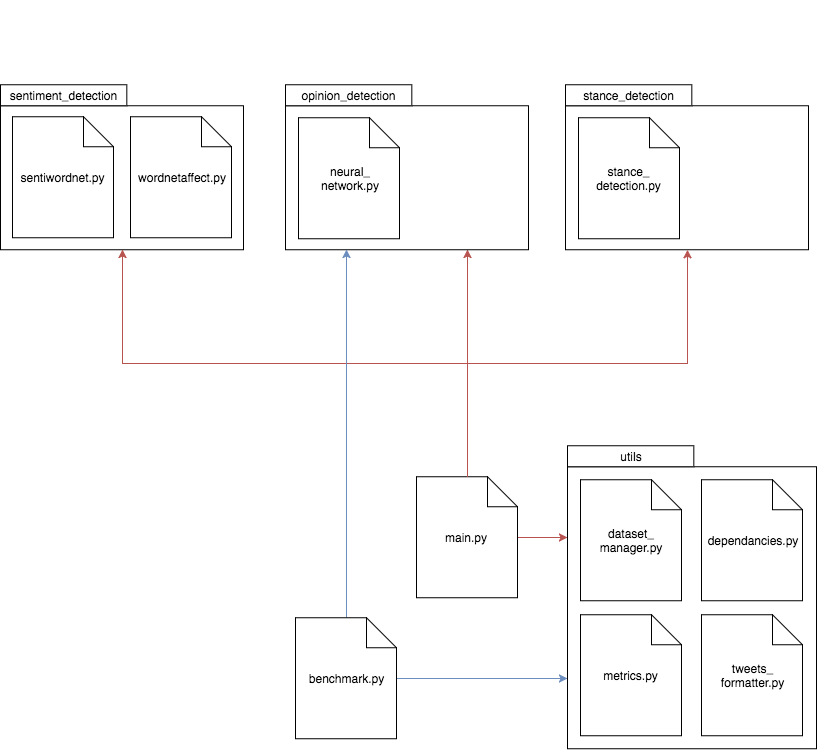
\includegraphics[width=\textwidth]{img/diagramme_package.png}}
	\caption{Diagramme de package}
\end{figure}
